\documentclass[aps,prl,reprint,superscriptaddress,longbibliography,floatfix]{revtex4-2}

\usepackage{amsmath,amssymb,bm}
\usepackage{booktabs}
\usepackage{graphicx}
\usepackage{microtype}
\usepackage{xcolor}
\usepackage[colorlinks=true,citecolor=blue!55!black,linkcolor=blue!55!black,urlcolor=blue!55!black]{hyperref}
\hypersetup{pdftitle={Response-Complex Memory in Exactly Degenerate Quantum Matter},pdfauthor={Thomas J. Wang; OKongOYangO},pdfsubject={Hodge-resolved quantum geometry and chaos under exact degeneracy}}

\graphicspath{{figures/}}
% Generated from audited v7 inference; do not edit.
\newif\ifheldoutcomplete
\heldoutcompletetrue
\newcommand{\HeldoutAbstract}{Exactly degenerate quantum manifolds have no internal level statistics, but their projectors move over coupling space. We formulate this motion as a response complex and compare one-sided frustration-free constraints with the orthogonal exact/coexact response of charge-resolved cubic $\mathcal N=2$ Sachdev--Ye--Kitaev cohomology. In the sequential $N=8,10,12$ pilot, 12 of 12 size/sector/panel groups reject both registered separable covariance nulls. A prediction sealed before the held-out $N=14$ opening is rejected by both nulls for the central/adjacent sparse pair, establishing structured four-point memory beyond the frozen separable Hodge-covariance law, without claiming complete entrywise covariance matching.}
\newcommand{\HeldoutBranch}{cohomological\_non\_gaussian\_class}
\newcommand{\HeldoutResultSentence}{The held-out adjacent and central medians are 0.301529 and 0.374993; their complete-realization confidence intervals do not overlap either sealed covariance prediction.}
\newcommand{\PilotResultSentence}{Across the complete $N=8,10,12$ pilot, 12 of 12 groups reject both registered separable covariance nulls under complete-realization resampling.}
\newcommand{\HeldoutSeal}{fc300dc7e4bd}
\newcommand{\HeldoutAdjacentObserved}{0.301529}
\newcommand{\HeldoutAdjacentPhysical}{$[0.291527,\,0.312061]$}
\newcommand{\HeldoutAdjacentCollapsed}{$[0.111789,\,0.111852]$}
\newcommand{\HeldoutAdjacentHodge}{$[0.112344,\,0.112513]$}
\newcommand{\HeldoutCentralObserved}{0.374993}
\newcommand{\HeldoutCentralPhysical}{$[0.368980,\,0.380473]$}
\newcommand{\HeldoutCentralCollapsed}{$[0.111338,\,0.111353]$}
\newcommand{\HeldoutCentralHodge}{$[0.111333,\,0.111348]$}

\newcommand{\Tr}{\operatorname{Tr}}
\newcommand{\dd}{\mathrm d}
\newcommand{\cH}{\mathcal H}
\newcommand{\cM}{\mathcal M}

\begin{document}

\title{Response-Complex Memory in Exactly Degenerate Quantum Matter}

\author{Thomas J. Wang}
\email{WangTheoPhys@outlook.com}
\affiliation{Tsinghua University, Beijing 100084, China}

\author{OKongOYangO}
\affiliation{The Pennsylvania State University, University Park, Pennsylvania 16802, USA}

\date{\today}

\begin{abstract}
\ifheldoutcomplete
\HeldoutAbstract
\else
This source tree freezes the response-complex formalism and the prediction protocol before the held-out calculation is opened. The result-bearing abstract is generated only after a valid prediction seal, explicit unseal, and fail-closed inference audit exist. No held-out scientific branch is claimed in this draft state.
\fi
\end{abstract}

\maketitle

\section{Spectral silence and response complexity}
\label{sec:introduction}

Exact degeneracy removes the level spacings on which conventional quantum-chaos diagnostics are built. If a protected multiplet contains \(D\) states at the same energy, its raw energy spectral form factor is constant and its connected form factor vanishes. This is a structural blind spot in supersymmetric sectors, frustration-free zero-mode manifolds, and other problems where lifting the degeneracy would destroy the object of interest. The missing information is carried by the motion of the protected projector \(P(\bm\lambda)\) over a coupling or moduli space, through its non-Abelian Berry curvature and quantum metric \cite{berry1984,wilczekzee1984,provostvallee1980,kato1950}.

Random-matrix-like Berry curvature in supersymmetric black-hole microstates and in generic \(\mathcal N=2\) Sachdev--Ye--Kitaev (SYK) models is already established \cite{chen2026berry,chen2024bps}. The question addressed here is different. Does random-matrix-like local curvature exhaust the information in the protected response, or do higher gauge-invariant correlations retain the mechanism by which the degeneracy is protected? Equivalently, can a two-point law predict a four-point response observable across distinct protection mechanisms? We compare one-sided positive-constraint Laughlin parents with a two-sided supersymmetric cohomology. The comparison uses the same covariance-whitened four-channel statistic, the same complete-realization uncertainty unit, and a prediction constructed before the held-out four-point outcome is opened.

The organizing object is a \emph{response complex}. For a frustration-free parent \(H=B^\dagger B\), the zero-mode response is one-sided. For \(H=\{Q,Q^\dagger\}\) with \(Q^2=0\), it decomposes into orthogonal exact and coexact branches. Their weights, covariance spectra, and effective ranks form a safe Hodge signature that is available without reading the four-channel outcome. We ask whether this signature selects a finite-size Gaussian response law. Coverage would support a two-point-controlled form of Geometric ETH; reproducible rejection would instead identify response-complex memory beyond that law. The protocol retains either outcome rather than fitting the held-out statistic after the fact.

\section{Hodge-resolved protected response}
\label{sec:response-complex}

The generic cubic \(\mathcal N=2\) SYK supercharge is
\begin{equation}
 \begin{split}
 Q(C)&=\sum_{i<j<k}C_{ijk}\psi_i\psi_j\psi_k,\qquad Q^2=0,\\
 H&=\{Q,Q^\dagger\}.
 \end{split}
 \label{eq:supercharge}
\end{equation}
In charge sector \(r\), the protected fiber is the harmonic cohomology
\begin{equation}
 \cH_{\mathrm{BPS},r}=\ker Q_r\cap\ker Q_{r-3}^\dagger.
 \label{eq:harmonic-fiber}
\end{equation}
We use generic isotropic complex three-forms \(C\), rather than the decomposable locus, because the generic BPS states are fortuitous and concentrated near the central charge sectors \cite{fu2017susy,chang2024fortuity}.

Let \(P\) project onto Eq.~\eqref{eq:harmonic-fiber}, and let \(H_\perp^+\) be the inverse of \(H\) on its positive-energy complement. For a real coupling tangent represented by \(\delta Q+\delta Q^\dagger\), the complement-to-fiber response is
\begin{align}
 X(\delta C)&=-H_\perp^+\left(Q\,\delta Q^\dagger+Q^\dagger\delta Q\right)P
 \nonumber\\
 &=X_-\oplus X_+,
 \label{eq:hodge-response}\\
 X_-&=-H_\perp^+Q\,\delta Q^\dagger P,
 \qquad
 X_+=-H_\perp^+Q^\dagger\delta QP.
 \nonumber
\end{align}
Nilpotency implies \(\operatorname{im}Q\perp\operatorname{im}Q^\dagger\), hence \(X_-^\dagger X_+=0\). We verify Eq.~\eqref{eq:hodge-response} against the direct resolvent derivative and a centered finite difference of \(P\). This identity turns the qualitative distinction between constraint and cohomological protection into a measurable branch structure.

The response is the quantum geometry, not an auxiliary diagnostic. In a local frame of the protected fiber, the matrix-valued quantum geometric tensor, metric, and Berry curvature are
\begin{equation}
 \begin{aligned}
 \mathcal Q_{ab}&=X_a^\dagger X_b,\qquad
 g_{ab}=\frac{\mathcal Q_{ab}+\mathcal Q_{ba}}{2},\\
 F_{ab}&=i\left(\mathcal Q_{ab}-\mathcal Q_{ba}\right).
 \end{aligned}
 \label{eq:qgt-response}
\end{equation}
Thus all gauge-invariant contractions used below are correlations of the same complement-resolved amplitudes that generate \(g\) and \(F\). For a one-sided parent \(H=B^\dagger B\) with \(BP=0\), the corresponding derivative is \(X=-H_\perp^+B^\dagger\delta B P\) and lies in a single response branch. Equation~\eqref{eq:hodge-response} is therefore an independent, two-sided protection mechanism rather than a change of basis within the Laughlin construction.

For an eight-channel tangent panel, define branch weights and Hodge balance by
\begin{equation}
 T_\pm=\sum_{a=1}^{8}\lVert X_{a,\pm}\rVert_F^2,
 \qquad
 \eta_H=\frac{4T_+T_-}{(T_++T_-)^2}.
 \label{eq:hodge-balance}
\end{equation}
The pre-outcome signature also contains branch-resolved channel, target, and complement covariance spectra. The collapsed null discards the branch label, whereas the Hodge null samples the two branches independently and forms their orthogonal direct sum. Both are parameter-free once the safe two-point data are fixed.

After complete channel whitening, the physical diagnostic is the gauge-invariant tensor
\begin{equation}
 \mathcal T_{abcd}=\frac{1}{D}\Tr\!\left(
 \widehat X_a^\dagger\widehat X_b
 \widehat X_c^\dagger\widehat X_d\right),
 \label{eq:four-channel}
\end{equation}
and its normalized Frobenius distance from the registered Gaussian Wick contraction. Independent target and complement basis rotations leave Eq.~\eqref{eq:four-channel} unchanged. The label ``non-Gaussian class'' below refers operationally to rejection of these frozen separable covariance models; it does not assert that the complete entrywise covariance operator has been matched.

\section{Sequential and sealed protocol}
\label{sec:protocol}

We study central \(r=N/2\) and adjacent \(r=N/2-1\) sectors at even \(N\). Each coupling realization supplies a sparse coordinate panel and an independent isotropic panel, both projected away from the complex radial line and orthonormalized before any four-channel result is inspected. The complete disorder realization is the uncertainty unit: tangent entries and tensor components are never resampled as independent observations.

The sequential pilot uses \(N=8,10,12\). Each realization is split into a safe metadata/array checkpoint and an outcome sidecar. The safe checkpoint contains the BPS rank, positive gap, numerical residuals, Hodge signature, covariance spectra, seeds, and source hashes, but no four-channel value. Per-realization Gaussian banks are generated from this safe file. A null replicate selects one bank draw per realization and takes their median; the physical uncertainty is a nonparametric bootstrap of complete-realization medians.

The held-out \(N=14\) computation is more restrictive. All safe response and null checkpoints must pass before the collapsed and Hodge numerical prediction intervals are written atomically. The prediction JSON is sealed by SHA-256. No scheduler dependency invokes the unseal command. Only a separate explicit action may validate the seal, open the sidecars, and score the central/adjacent sparse pair. The isotropic pair is secondary and cannot change the primary branch.

The registered branches are: simultaneous coverage by both nulls; coverage only by the Hodge null; rejection of both with reproducible response memory; statistical indistinguishability from the decomposable structured control; or feasibility failure. A decomposable three-form recovers exact curvature atoms \(0,\pm\alpha^{-2}\) with analytic multiplicities, and a one-sided synthetic response reproduces the accepted Laughlin Gaussian null exactly. These controls test the algebra and implementation independently of the generic-coupling outcome.

\section{Response-complex inference}
\label{sec:results}

\PilotResultSentence

\ifheldoutcomplete
\begin{figure*}[t]
 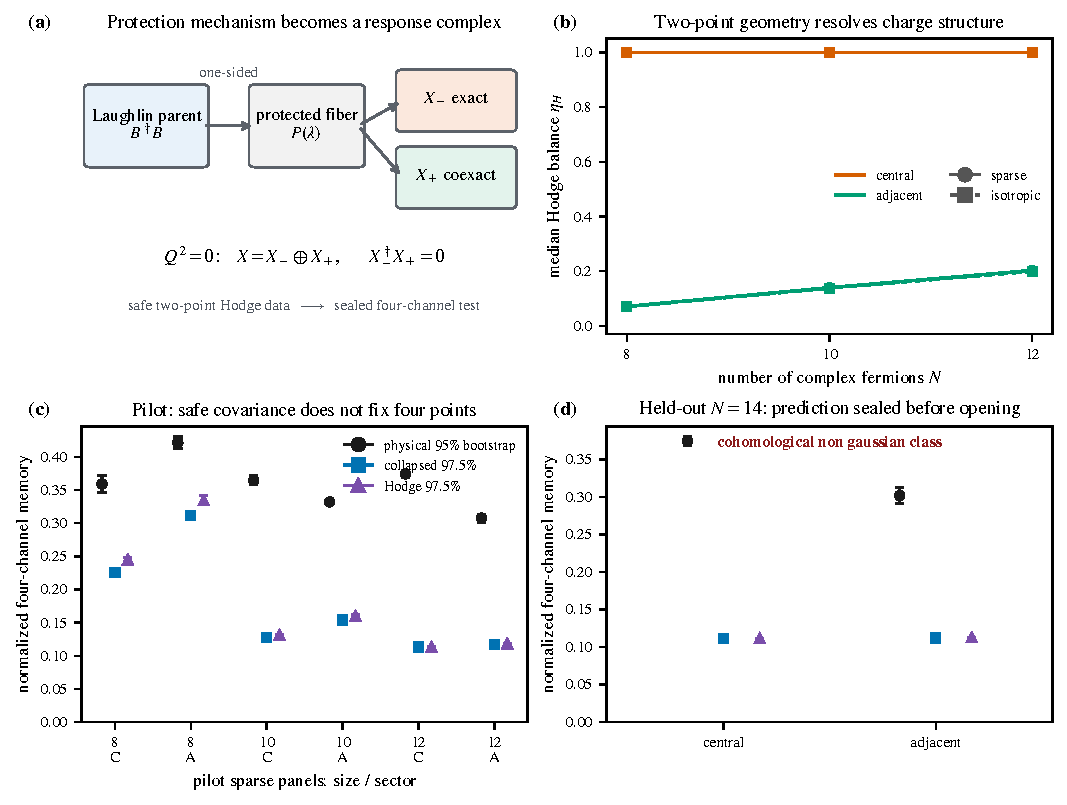
\includegraphics[width=\textwidth]{figure_susy_hodge_geometric_eth_v7.pdf}
 \caption{\textbf{Hodge-resolved response-complex test.} The panels show the one-sided/two-sided protection map, charge-resolved Hodge balance, complete-realization pilot intervals, and the sealed \(N=14\) central/adjacent sparse validation. Every plotted scalar is recoverable from the associated hash manifest.}
 \label{fig:hodge-inference}
\end{figure*}

\HeldoutResultSentence The frozen decision therefore selects structured cohomological response memory beyond the registered separable covariance laws. Figure~\ref{fig:hodge-inference} separates the exact two-point Hodge structure from the higher response memory tested by Eq.~\eqref{eq:four-channel}; the exact branch identifier and prediction hash are retained in the audited Supplemental Material and machine-readable artifact.
\else
The result-bearing figure and paragraph are disabled until the prediction seal, unsealed aggregate, and inference artifact pass the delivery audit. This fail-closed draft cannot state a held-out branch.
\fi

\section{Discussion}
\label{sec:discussion}

The response-complex construction changes the object being classified. Spectral chaos asks how eigenvalues fluctuate after a degeneracy is resolved. Here the protected energies remain exactly equal, and the diagnostic asks how the degenerate fiber moves over coupling space. Equation~\eqref{eq:qgt-response} makes the replacement exact: two-point response generates the quantum metric and Berry curvature, while Eq.~\eqref{eq:four-channel} tests whether their underlying amplitudes obey a Gaussian higher-moment closure. The exact/coexact split supplies a mechanism-level coordinate on that motion. One-sided positive constraints and two-sided cohomology need not share the same higher response law even when their local curvature spectra are random-matrix-like.

The claim is deliberately finite-size and geometric. It is not conventional ETH, thermalization, a real-time chaos diagnostic, or a thermodynamic theorem. In particular, a successful sealed finite-size prediction would establish covariance-controlled Geometric ETH only on the tested sequence; it would not supply an asymptotic concentration law. Conversely, rejection localizes the missing information above the registered separable two-point structure without proving that every more general Gaussian covariance model fails. Generic \(\mathcal N=2\) SYK supplies a genuinely supersymmetric protection mechanism but not spatial locality. Establishing locality universality requires a later nilpotent lattice-supercharge model with a fixed charge-resolved zero-mode count, an open gap, and a nontrivially moving harmonic projector \cite{huijse2009cohomology,zhang2024local}.

There is also a covariance boundary. The collapsed and Hodge nulls match the registered marginal covariance data under a separable matrix-normal ansatz. If they are rejected, the result establishes structured memory beyond that ansatz. A stronger statement of intrinsic non-Gaussianity would require matching or independently constraining the complete nonseparable entrywise covariance operator. This distinction is not a weakness of the sealed test; it identifies the next theoretical target without allowing a post-outcome refit to rewrite the primary result.


\begin{acknowledgments}
The numerical artifacts, complete-realization resampling records, source hashes, and prediction seals are retained with the reproducibility package. We thank the Quantum Harness community for discussions motivating fail-closed computational tests.
\end{acknowledgments}

\bibliography{references}

\end{document}
